\newpage
\subsection{Caso d'uso UC8 - Visualizzazione API acquistate}
\label{UC8}
\begin{figure}[ht]
	\centering
	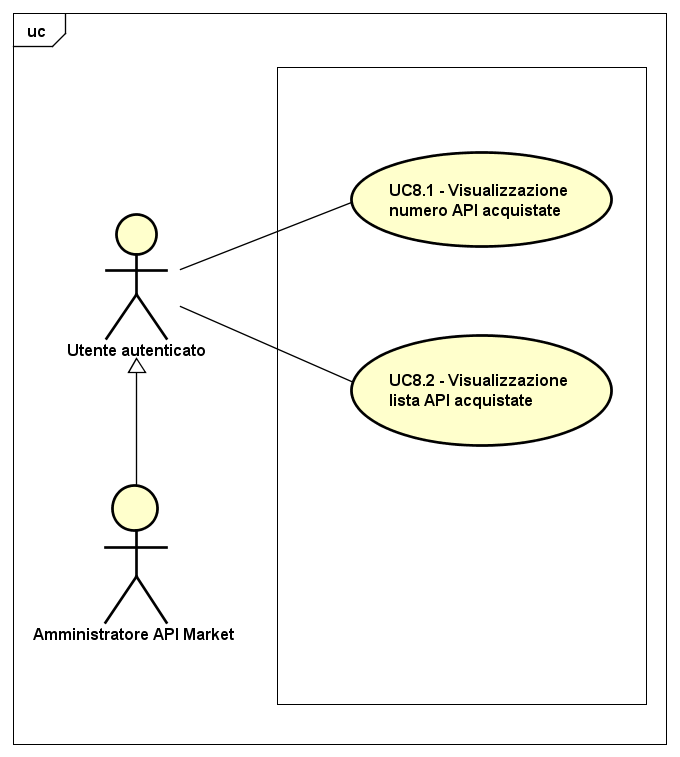
\includegraphics[scale=0.45]{UML/UC8.png}
	\caption{UC8: Visualizzazione API}
\end{figure}

\begin{longtable}{ l | p{11cm}}
	\hline
	\rowcolor{Gray}
	\multicolumn{2}{c}{UC8 - Visualizzazione API acquistate}\\
	\hline
	 \textbf{Attori} & Utente autenticato, Amministratore API Market \\
	\textbf{Descrizione} & L'attore visualizza le API da lui acquistate \\
	\textbf{Pre-Condizioni} & L'attore ha scelto di visualizzare le API da lui acquistate \\
	\textbf{Post-Condizioni} & L'attore ha visualizzato le API da lui acquistate \\
	\textbf{Scenario Principale} & 
	\begin{enumerate*}[label=(\arabic*.),itemjoin={\newline}]
		\item L'attore può visualizzare il numero delle API acquistate e attive (UC8.1)
		\item L'attore può visualizzare la lista delle API acquistate e attive (UC8.2)
	\end{enumerate*}\\
	\textbf{Scenari Alternativi} & 
	\begin{enumerate*}[label=(\arabic*.),itemjoin={\newline}]
		\item L'attore può visualizzare i dati relativi ad una singola API (UC7)
	\end{enumerate*}\\
\end{longtable}

\subsubsection{Caso d'uso UC8.1: Visualizzazione numero API acquistate}
\label{UC8_1}

\begin{minipage}{\linewidth}
	\begin{tabular}{ l | p{11cm}}
		\hline
		\rowcolor{Gray}
		\multicolumn{2}{c}{UC8.1 - Visualizzazione numero API acquistate} \\
		\hline
		\textbf{Attori} & Utente autenticato, Amministratore API Market \\
		\textbf{Descrizione} & L'attore visualizza il numero di API da lui acquistate \\
		\textbf{Pre-Condizioni} & L'attore si trova nella schermata di visualizzazione API acquistate \\
		\textbf{Post-Condizioni} & L'attore ha visualizzato il numero delle API da lui acquistate \\
		\textbf{Scenario Principale} & 
		\begin{enumerate*}[label=(\arabic*.),itemjoin={\newline}]
			\item L'attore può visualizzare il numero di API acquistate
		\end{enumerate*}\\
	\end{tabular}
\end{minipage}

\newpage
\subsubsection{Caso d'uso UC8.2: Visualizzazione lista API acquistate}
\label{UC8_2}
\begin{figure}[ht]
	\centering
	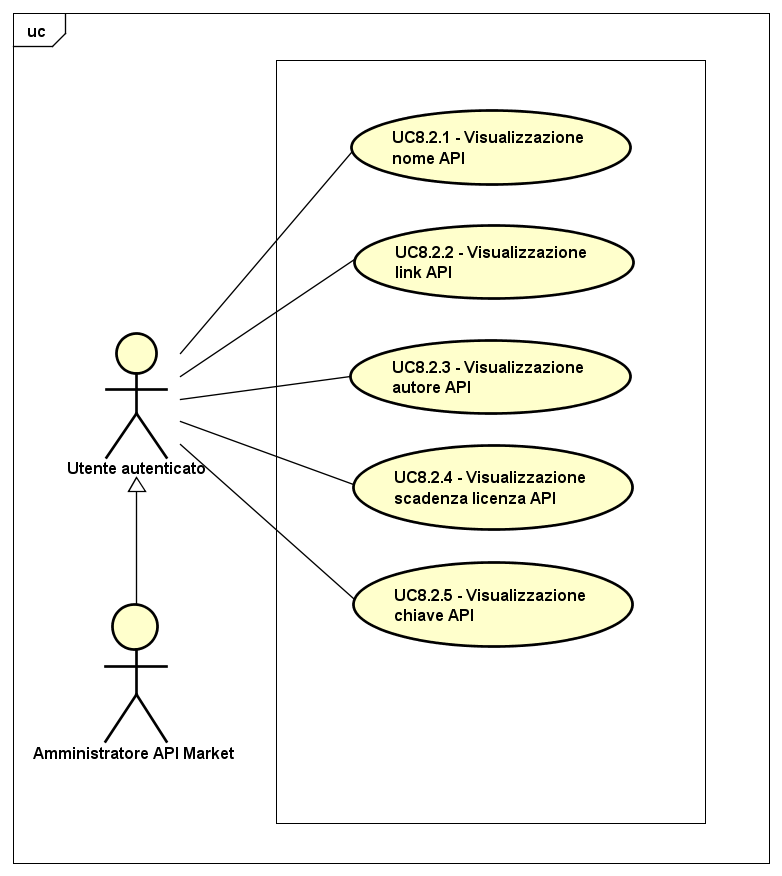
\includegraphics[scale=0.45]{UML/UC8_2.png}
	\caption{UC8.2: Visualizzazione lista API acquistate}
\end{figure}

\begin{minipage}{\linewidth}
	\begin{tabular}{ l | p{11cm}}
		\hline
		\rowcolor{Gray}
		\multicolumn{2}{c}{UC8.2 - Visualizzazione lista API acquistate} \\
		\hline
		\textbf{Attori} & Utente autenticato, Amministratore API Market \\
		\textbf{Descrizione} & L'attore visualizza la lista delle API da lui acquistate \\
		\textbf{Pre-Condizioni} & L'attore si trova nella schermata di visualizzazione API acquistate \\
		\textbf{Post-Condizioni} & L'attore ha visualizzato la lista delle API da lui acquistate \\
		\textbf{Scenario Principale} & 
		\begin{enumerate*}[label=(\arabic*.),itemjoin={\newline}]
			\item L'attore può visualizzare il nome dell'API (UC8.2.1)
			\item L'attore può visualizzare il link alla pagina di visualizzazione API (UC8.2.2)
			\item L'attore può visualizzare il nome dell'autore dell'API (UC8.2.3)
			\item L'attore può visualizzare la data di scadenza della propria licenza per l'API (UC8.2.4)
			\item L'attore può visualizzare la propria chiave per l'API (UC8.2.5)
		\end{enumerate*}\\
	\end{tabular}
\end{minipage}

\paragraph{Caso d'uso UC8.2.1: Visualizzazione nome API}
\label{UC8_2_1}

\begin{minipage}{\linewidth}
	\begin{tabular}{ l | p{11cm}}
		\hline
		\rowcolor{Gray}
		\multicolumn{2}{c}{UC8.2.1 - Visualizzazione nome API} \\
		\hline
		\textbf{Attori} & Utente autenticato, Amministratore API Market \\
		\textbf{Descrizione} & L'attore visualizza nella lista il nome dell'API \\
		\textbf{Pre-Condizioni} & L'attore si trova nella schermata di visualizzazione API acquistate \\
		\textbf{Post-Condizioni} & L'attore ha visualizzato nella lista il nome dell'API \\
		\textbf{Scenario Principale} & 
		\begin{enumerate*}[label=(\arabic*.),itemjoin={\newline}]
			\item L'attore può visualizzare nella lista il nome dell'API
		\end{enumerate*}\\
	\end{tabular}
\end{minipage}

\paragraph{Caso d'uso UC8.2.2: Visualizzazione link API}
\label{UC8_2_2}

\begin{minipage}{\linewidth}
	\begin{tabular}{ l | p{11cm}}
		\hline
		\rowcolor{Gray}
		\multicolumn{2}{c}{UC8.2.2 - Visualizzazione link API} \\
		\hline
		\textbf{Attori} & Utente autenticato, Amministratore API Market \\
		\textbf{Descrizione} & L'attore visualizza nella lista il link alla visualizzazione dell'API \\
		\textbf{Pre-Condizioni} & L'attore si trova nella schermata di visualizzazione dell'API acquistate \\
		\textbf{Post-Condizioni} & L'attore ha visualizzato nella lista il link alla visualizzazione dell'API \\
		\textbf{Scenario Principale} & 
		\begin{enumerate*}[label=(\arabic*.),itemjoin={\newline}]
			\item L'attore può visualizzare nella lista il link alla visualizzazione dell'API
		\end{enumerate*}\\
	\end{tabular}
\end{minipage}

\paragraph{Caso d'uso UC8.2.4: Visualizzazione scadenza licenza}
\label{UC8_2_4}

\begin{minipage}{\linewidth}
	\begin{tabular}{ l | p{11cm}}
		\hline
		\rowcolor{Gray}
		\multicolumn{2}{c}{UC8.2.3 - Visualizzazione scadenza licenza} \\
		\hline
		\textbf{Attori} & Utente autenticato, Amministratore API Market \\
		\textbf{Descrizione} & L'attore visualizza nella lista la data di scadenza della propria licenza per l'API \\
		\textbf{Pre-Condizioni} & L'attore si trova nella schermata di visualizzazione API acquistate \\
		\textbf{Post-Condizioni} & L'attore ha visualizzato nella lista la data di scadenza dell'API \\
		\textbf{Scenario Principale} & 
		\begin{enumerate*}[label=(\arabic*.),itemjoin={\newline}]
			\item L'attore può visualizzare nella lista la data di scadenza della propria licenza per l'API
		\end{enumerate*}\\
	\end{tabular}
\end{minipage}

\paragraph{Caso d'uso UC8.2.5: Visualizzazione chiave API}
\label{UC8_2_5}

\begin{minipage}{\linewidth}
	\begin{tabular}{ l | p{11cm}}
		\hline
		\rowcolor{Gray}
		\multicolumn{2}{c}{UC8.2.5 - Visualizzazione chiave API} \\
		\hline
		\textbf{Attori} & Utente autenticato, Amministratore API Market \\
		\textbf{Descrizione} & L'attore visualizza nella lista la propria chiave di utilizzo per l'API \\
		\textbf{Pre-Condizioni} & L'attore si trova nella schermata di visualizzazione API acquistate \\
		\textbf{Post-Condizioni} & L'attore ha visualizzato nella lista la propria chiave di utilizzo per l'API \\
		\textbf{Scenario Principale} & 
		\begin{enumerate*}[label=(\arabic*.),itemjoin={\newline}]
			\item L'attore può visualizzare nella lista la propria chiave di utilizzo per l'API
		\end{enumerate*}\\
	\end{tabular}
\end{minipage}